\documentclass[aspectratio=169,t]{beamer}

\usetheme{default}
\usecolortheme{default}

\definecolor{darkblue}{RGB}{15,40,80}
\definecolor{midblue}{RGB}{30,80,160}
\definecolor{lightblue}{RGB}{200,220,245}
\definecolor{accent}{RGB}{220,80,40}
\definecolor{dkgreen}{RGB}{30,130,70}
\definecolor{gold}{RGB}{180,140,0}
\definecolor{lightgray}{RGB}{240,242,246}
\definecolor{purple}{RGB}{120,40,160}

\setbeamercolor{frametitle}{fg=white,bg=darkblue}
\setbeamercolor{title}{fg=white}
\setbeamercolor{subtitle}{fg=lightblue}
\setbeamercolor{author}{fg=lightblue}
\setbeamercolor{normal text}{fg=darkblue}
\setbeamercolor{block title}{fg=white,bg=midblue}
\setbeamercolor{block body}{fg=darkblue,bg=lightblue!40}
\setbeamercolor{alerted text}{fg=accent}
\setbeamercolor{example text}{fg=dkgreen}
\setbeamercolor{structure}{fg=midblue}
\setbeamercolor{itemize item}{fg=accent}
\setbeamercolor{itemize subitem}{fg=midblue}
\setbeamercolor{enumerate item}{fg=accent}

\setbeamerfont{frametitle}{size=\large,series=\bfseries}
\setbeamerfont{title}{size=\LARGE,series=\bfseries}
\setbeamerfont{block title}{series=\bfseries}

\setbeamertemplate{navigation symbols}{}
\setbeamertemplate{itemize item}{\small\raise0.5pt\hbox{$\bullet$}}
\setbeamertemplate{itemize subitem}{\small\raise0.5pt\hbox{$\circ$}}
\setbeamertemplate{frametitle}[default][center]
\setbeamertemplate{footline}{%
  \hfill\usebeamerfont{footline}\color{darkblue!50}%
  \insertframenumber/\inserttotalframenumber\hspace{4pt}\vspace{4pt}}

\usepackage{amsmath,amssymb}
\usepackage{booktabs}
\usepackage{xcolor}
\usepackage{colortbl}
\usepackage{tikz}
\usetikzlibrary{arrows.meta,positioning,shapes.geometric,fit,backgrounds,calc,decorations.pathreplacing}
\usepackage{pgfplots}
\pgfplotsset{compat=1.16}
\usepackage{array}

\newcommand{\pw}{\mathrm{pw}}
\newcommand{\Bell}{\mathrm{Bell}}
\newcommand{\nb}{n_{\mathrm{back}}}
\newcommand{\curr}{\texttt{curr}}

\title{Record Merging at Scale}
\subtitle{Hash Tables, Cache Hierarchies,\\Extendible Hashing, and Parallel Sort--Merge}
\author{Victor S.\ Miller}
\date{}

\begin{document}

% ==================== TITLE ====================
{
\setbeamercolor{background canvas}{bg=darkblue}
\begin{frame}[plain]
  \vspace{0.8cm}
  \begin{center}
    {\color{lightblue}\small\itshape Talk II of II}\\[0.5cm]
    {\color{white}\LARGE\bfseries Record Merging at Scale}\\[0.5cm]
    {\color{lightblue}\large Hash Tables, Cache Hierarchies,\\[3pt]
     Extendible Hashing, and Parallel Sort--Merge}\\[0.8cm]
    {\color{white}\large Victor S.\ Miller}\\[0.3cm]
    {\color{lightblue!70}\normalsize \today}
  \end{center}
\end{frame}
}

% ==================== OUTLINE ====================
\begin{frame}{Talk Outline}
\small
\begin{columns}[t]
\column{0.32\textwidth}
\textbf{\color{midblue}The Problem}
\begin{itemize}
  \item Where it arises
  \item The abstract merging problem
  \item Why it's hard at scale
\end{itemize}
\vspace{0.2cm}
\textbf{\color{midblue}Iteration 1: Linear Probing}
\begin{itemize}
  \item Design and performance
  \item Write-combining buffer
  \item Memory crisis at large $n$
\end{itemize}

\column{0.32\textwidth}
\textbf{\color{midblue}Iteration 2: Extendible Hashing}
\begin{itemize}
  \item EH (Fagin et al.\ 1979)
  \item The O(range) split fix
\end{itemize}
\vspace{0.2cm}
\textbf{\color{midblue}Iteration 3: Locality}
\begin{itemize}
  \item Radix-sort insertion buffer
  \item Hardware-adaptive constants
\end{itemize}
\vspace{0.2cm}
\textbf{\color{midblue}Iteration 4: OS Memory}
\begin{itemize}
  \item The malloc/free trap on macOS
\end{itemize}

\column{0.32\textwidth}
\textbf{\color{midblue}Iteration 5: Going Parallel}
\begin{itemize}\setlength{\itemsep}{1pt}
  \item Why hash-based parallelism failed
  \item Generate $\to$ sort $\to$ merge
  \item Merging by hash range
  \item Load balancing by randomising
  \item Effect of pruning (Du)
\end{itemize}
\vspace{0.05cm}
\textbf{\color{midblue}Results and Lessons}
\begin{itemize}
  \item $n=61$: 97\,min, $<$2\,GB (laptop)
  \item $n\le 75$: 768\,GB, 64 cores
  \item What still needs checking
\end{itemize}
\end{columns}
\end{frame}

% ==================== PART I: THE PROBLEM ====================
{
\setbeamercolor{background canvas}{bg=darkblue}
\begin{frame}[plain]
  \vspace{2cm}
  \begin{center}
    {\color{lightblue}\small Part I}\\[0.4cm]
    {\color{white}\LARGE\bfseries The Problem}
  \end{center}
\end{frame}
}

\begin{frame}{Where This Arose}
\begin{columns}[c]
\column{0.52\textwidth}
We were computing Hamiltonian paths in sparse graphs
using \textbf{frontier dynamic programming}: process
vertices one at a time; maintain a table of
(connectivity-state, count) pairs at each step.

\vspace{0.2cm}
\textbf{At each DP step:}
\begin{enumerate}
  \item Scan every entry $(k, c)$ in the current table
  \item Apply the current graph edge(s) to produce new states $k'$
  \item \alert{Many source states map to the same $k'$} — their counts must be summed
  \item The result table feeds the next step
\end{enumerate}

\vspace{0.2cm}
\begin{block}{Scale at $n=61$}
  Peak step: 620 million output states, each 24 bytes.\\
  Live data: $\approx 20$\,GB. Without the work in this talk:
  $>80$\,GB swap, computation killed by the OS.
\end{block}

\column{0.44\textwidth}
\textbf{But the problem is universal.}

\vspace{0.2cm}
The same \emph{stream-merge} pattern arises in:
\begin{itemize}
  \item \textbf{Map-Reduce} — the shuffle/reduce phase
  \item \textbf{Database joins} — hash aggregation
  \item \textbf{Graph analytics} — message passing in bulk-synchronous parallel
  \item \textbf{Compilers} — data-flow analysis fixpoints
  \item \textbf{Scientific DP} — any table-driven recurrence with collisions
\end{itemize}

\vspace{0.2cm}
\begin{exampleblock}{Abstract formulation}
  Given a stream of $(k, v)$ pairs: produce a table with
  one entry per distinct $k$, value $= \bigoplus_i v_i$
  for all pairs with that key. Operator $\oplus$ is
  commutative and associative (here: integer addition).
\end{exampleblock}
\end{columns}
\end{frame}

\begin{frame}{Why It's Hard at Scale}
\small
\begin{columns}[c]
\column{0.52\textwidth}
\textbf{Naïve approach:} hash table, accumulate-on-insert.
\begin{itemize}
  \item Hash $k$; if found, add $v$; else insert $(k,v)$
  \item Works until table exceeds L3 cache
\end{itemize}

\vspace{0.15cm}
\textbf{The fundamental tension:}

\begin{center}
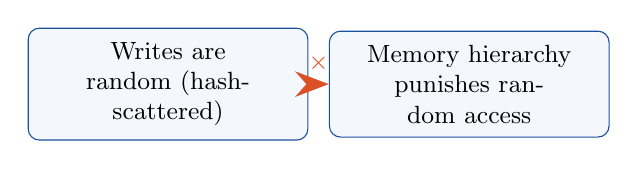
\begin{tikzpicture}[scale=0.85,
  box/.style={draw=midblue,fill=lightblue!20,rounded corners,inner sep=5pt,
              text width=3.2cm,align=center,font=\small}]
  \node[box] (w) at (0,0) {Writes are\\random (hash-scattered)};
  \node[box] (m) at (4.5,0) {Memory hierarchy\\punishes random access};
  \draw[-Stealth,thick,accent,line width=2pt] (w) -- node[above,font=\small]{$\times$} (m);
\end{tikzpicture}
\end{center}

\vspace{0.1cm}
100M states $\times$ 24B = 2.4\,GB table.\\
Each insert = 1 random DRAM access $\approx 100$\,ns.\\
100M inserts: \textbf{10 seconds minimum} from cache misses alone.

\column{0.44\textwidth}
\centering
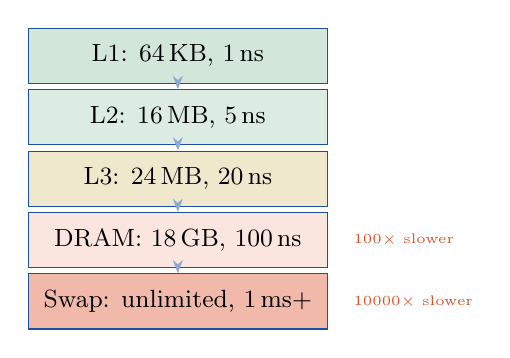
\begin{tikzpicture}[scale=0.78,
  box/.style={draw=midblue,fill=lightblue!20,minimum width=3.8cm,
              minimum height=0.7cm,font=\small,align=center}]
  \node[box,fill=dkgreen!20] (l1) at (0,4.2) {L1: 64\,KB, 1\,ns};
  \node[box,fill=dkgreen!15] (l2) at (0,3.2) {L2: 16\,MB, 5\,ns};
  \node[box,fill=gold!20] (l3) at (0,2.2) {L3: 24\,MB, 20\,ns};
  \node[box,fill=accent!15] (dr) at (0,1.2) {DRAM: 18\,GB, 100\,ns};
  \node[box,fill=accent!40] (sw) at (0,0.2) {Swap: unlimited, 1\,ms+};
  \foreach \a/\b in {l1/l2,l2/l3,l3/dr,dr/sw}{
    \draw[-Stealth,midblue!50] (\a.south) -- (\b.north);}
  \node[right=0.2cm,font=\tiny\color{accent}] at (dr.east) {$100\times$ slower};
  \node[right=0.2cm,font=\tiny\color{accent}] at (sw.east) {$10000\times$ slower};
\end{tikzpicture}

\vspace{0.2cm}
{\small Apple M3 Pro (our platform).\\
A 2.4\,GB table fits in DRAM but not L3.\\
A 20\,GB table at peak causes swap.}
\end{columns}
\end{frame}

% ==================== PART II: LINEAR PROBING ====================
{
\setbeamercolor{background canvas}{bg=darkblue}
\begin{frame}[plain]
  \vspace{2cm}
  \begin{center}
    {\color{lightblue}\small Part II}\\[0.4cm]
    {\color{white}\LARGE\bfseries Iteration 1: Linear Probing}
  \end{center}
\end{frame}
}

\begin{frame}{Linear-Probing Hash Table}
\small
\begin{columns}[c]
\column{0.52\textwidth}
\textbf{Structure:} flat \texttt{keys[cap]} and \texttt{vals[cap]}.
\begin{itemize}
  \item Key: \texttt{u64}; value: \texttt{u128} (path count)
  \item 24 bytes/slot; load factor 75\%
  \item Pre-allocated at $1.5\times$ expected input count
\end{itemize}

\vspace{0.15cm}
\textbf{Insert $(k, v)$:}
\begin{enumerate}\small
  \item $i = h(k) \bmod \texttt{cap}$
  \item Probe until \texttt{keys}[$i$] $= k$ (add $v$) or empty (insert)
\end{enumerate}

\vspace{0.1cm}
\textbf{Reset:} \texttt{memset(keys, 0)} — fast, sequential.

\vspace{0.1cm}
\begin{exampleblock}{Initial result for $n=57$}
  134\,s naive; 43\,s with MaxSAT+SA ordering.
\end{exampleblock}

\column{0.44\textwidth}
\begin{alertblock}{Two problems at scale}
  \textbf{1. Pre-allocation mismatch.}\\
  $n=59$ step 39: 118M in, 27M out.
  LP allocates $6.44$\,GB; only 6\% used.\\[4pt]
  \textbf{2. Three-table resize spike.}
  \begin{center}{\small
  \begin{tabular}{lrl}
  \texttt{curr} & 3.22\,GB & active \\
  old \texttt{nxt} & 3.22\,GB & rehashing \\
  new \texttt{nxt} & 6.44\,GB & \alert{new} \\
  \midrule
  Total & \alert{12.9\,GB} & simultaneous \\
  \end{tabular}}
  \end{center}
  On 18\,GB machine: OS triggers swap.
\end{alertblock}
\end{columns}
\end{frame}

\begin{frame}{Write-Combining Buffer}
\small
\begin{columns}[c]
\column{0.52\textwidth}
\textbf{Idea:} batch writes by hash region before hitting the table.

\vspace{0.1cm}
\begin{block}{Design}
$B=1024$ slots. Slot $b$ covers $[b\cdot\texttt{cap}/1024,\;(b{+}1)\cdot\texttt{cap}/1024)$.\\[2pt]
Each slot: FIFO of 16 entries = 384\,bytes. Fits in L1/L2.
\end{block}

\vspace{0.1cm}
\textbf{On insert $(k, v)$:}
\begin{enumerate}\small
  \item Scan slot for $k$ — merge if found (L1 hit)
  \item If room: append to slot buffer
  \item If full: flush 16 entries to table (warms 1.5\,MB region)
\end{enumerate}
Each 1.5\,MB region: loaded once, receives 16 writes.

\column{0.44\textwidth}
\begin{center}
\begin{tabular}{lrr}
\toprule
Step & Before & After \\
\midrule
$n=58$ step 28 & 7.6\,s & 4.3\,s \\
$n=58$ step 38 & 74.2\,s & 33.4\,s \\
$n=58$ step 40 & 41.8\,s & 21.5\,s \\
\midrule
$n=58$ full run & 265.8\,s & \textbf{149.4\,s} \\
\bottomrule
\end{tabular}
\end{center}

\vspace{0.2cm}
\begin{alertblock}{But only delays the problem}
  $n=59$: table is 9.7\,GB; flush region 9.5\,MB — still cold DRAM.\\[3pt]
  $n=59$ step 38 under LP: \textbf{853 seconds}.
\end{alertblock}
\end{columns}
\end{frame}

% ==================== PART III: EH ====================
{
\setbeamercolor{background canvas}{bg=darkblue}
\begin{frame}[plain]
  \vspace{2cm}
  \begin{center}
    {\color{lightblue}\small Part III}\\[0.4cm]
    {\color{white}\LARGE\bfseries Iteration 2: Extendible Hashing}
  \end{center}
\end{frame}
}

\begin{frame}{Extendible Hashing [Fagin, Nievergelt, Pippenger, Strong 1979]}
\begin{columns}[c]
\column{0.52\textwidth}
\textbf{Key property:} the table grows \emph{proportional to its contents},
not its input. No pre-allocation; no resize spikes.

\vspace{0.15cm}
\textbf{Three components:}
\begin{enumerate}
  \item \textbf{Bucket} ($B=32$ entries, 776\,bytes):\\
        Key-value pairs + count + local depth.\\
        Entire bucket fits in L1 cache.
  \item \textbf{Slab pool} (bump allocator):\\
        4096-bucket slabs, $\approx 3.2$\,MB each.\\
        Reset = rewind usage counter.
  \item \textbf{Directory} \texttt{dir[$0\ldots 2^{gd}$-1]}:\\
        Top $gd$ hash bits $\to$ bucket pointer.
\end{enumerate}

\vspace{0.15cm}
\textbf{Insert:} hash top $gd$ bits $\to$ scan bucket (L1);
accumulate if found; insert if room; split if full.

\column{0.44\textwidth}
\centering
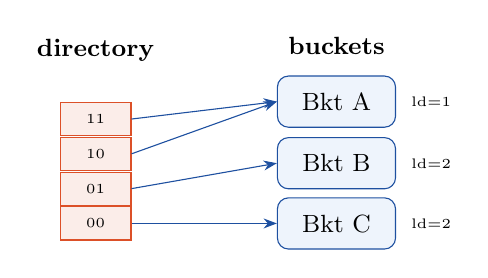
\begin{tikzpicture}[scale=0.85,
  bkt/.style={draw=midblue,fill=lightblue!30,rounded corners,
              minimum width=1.5cm,minimum height=0.65cm,font=\small},
  dir/.style={draw=accent,fill=accent!10,minimum width=0.9cm,
              minimum height=0.42cm,font=\tiny}]
  \foreach \i/\lbl in {0/00,1/01,2/10,3/11}{
    \node[dir] (d\i) at (0,\i*0.52) {\lbl};}
  \node[above=2pt,font=\small\bfseries] at (0,2.2) {directory};
  \node[bkt] (b0) at (3.6,1.82) {Bkt A};
  \node[bkt] (b1) at (3.6,0.9) {Bkt B};
  \node[bkt] (b2) at (3.6,0.0) {Bkt C};
  \draw[-Stealth,midblue] (d3.east) -- (b0.west);
  \draw[-Stealth,midblue] (d2.east) -- (b0.west);
  \draw[-Stealth,midblue] (d1.east) -- (b1.west);
  \draw[-Stealth,midblue] (d0.east) -- (b2.west);
  \node[font=\small\bfseries,above=2pt] at (3.6,2.3) {buckets};
  \node[font=\tiny,right=2pt] at (b0.east) {ld=1};
  \node[font=\tiny,right=2pt] at (b1.east) {ld=2};
  \node[font=\tiny,right=2pt] at (b2.east) {ld=2};
\end{tikzpicture}

\vspace{0.2cm}
\textbf{Proportional allocation:}\\
Memory $\propto$ \emph{actual content}, not input estimate.
No pre-allocation waste. No resize spike.

\vspace{0.1cm}
{\small Originally designed for disk pages (1979). Same principle applies
to DRAM$\to$L3 in 2025.}
\end{columns}
\end{frame}

\begin{frame}{The O(range) Split Fix}
\small
\begin{columns}[t]
\column{0.50\textwidth}
\textbf{Split} when bucket $b$ at \texttt{dir}[$i$] is full:
\begin{enumerate}\small
  \item \texttt{ld} $=$ $gd$: double directory
  \item Increment \texttt{ld}; allocate sibling $b'$
  \item Redistribute by hash bit $64 - \texttt{ld}$
  \item \alert{Update directory entries pointing to $b$}
\end{enumerate}

\vspace{0.15cm}
\textbf{Naïve step 4:} scan all $2^{gd}$ entries.\\
$gd=18$: $141\text{K}\times 262\text{K} = \mathbf{37\times10^9}$ iterations/step. \alert{$10\times$ regression}.

\vspace{0.15cm}
\begin{exampleblock}{O(range) fix}
Entries for $b$ form a \textbf{contiguous aligned range}:
\[
  \textit{range} = 2^{gd-\texttt{ld}},\quad
  \textit{base} = i\;\&\;(\sim(\textit{range}-1))
\]
Redirect $[\textit{base}+\textit{range}/2,\;\textit{base}+\textit{range})$ to $b'$.\\
At $\texttt{ld}=gd-1$: $O(1)$/split. \textbf{Total: $O(N/B)$ amortised.}
\end{exampleblock}

\column{0.46\textwidth}
\begin{alertblock}{Why the write buffer fails for EH}
  LP slot $b$: \emph{contiguous} region — one flush warms it in L3.\\[4pt]
  EH buckets: allocated in \emph{insertion order}. Slot $b$'s 1024 entries point to 1024 \emph{scattered} buckets.\\[4pt]
  Each flush: 1024 cold DRAM loads regardless.\\[4pt]
  \textbf{Result:} $1.20\times$ speedup on EH vs.\ $1.78\times$ on LP.
\end{alertblock}
\end{columns}
\end{frame}

% ==================== PART IV: LOCALITY ====================
{
\setbeamercolor{background canvas}{bg=darkblue}
\begin{frame}[plain]
  \vspace{2cm}
  \begin{center}
    {\color{lightblue}\small Part IV}\\[0.4cm]
    {\color{white}\LARGE\bfseries Iteration 3: Locality at Scale}
  \end{center}
\end{frame}
}

\begin{frame}{Radix-Sort Insertion Buffer}
\small
\begin{columns}[c]
\column{0.52\textwidth}
\textbf{Root cause:} EH directory entries for a hash prefix point to \emph{non-contiguous} buckets.

\vspace{0.1cm}
\textbf{Fix:} sort outputs by hash prefix \emph{before} inserting.

\vspace{0.1cm}
\begin{block}{Radix-sort buffer}
  $P=2^R$ slots. Slot $b$ collects outputs where $h(k')\gg(64-R)=b$.\\[2pt]
  \textbf{Collect:} append $(k',v')$ to slot $b$ — $O(1)$.\\[2pt]
  \textbf{Flush:} slots $0\ldots P-1$ in order. All entries in slot $b$ target directory range $[b\cdot2^{gd-R},\;(b{+}1)\cdot2^{gd-R})$.\\[2pt]
  Each EH bucket loaded from DRAM \textbf{exactly once}.
\end{block}

\column{0.44\textwidth}
\centering
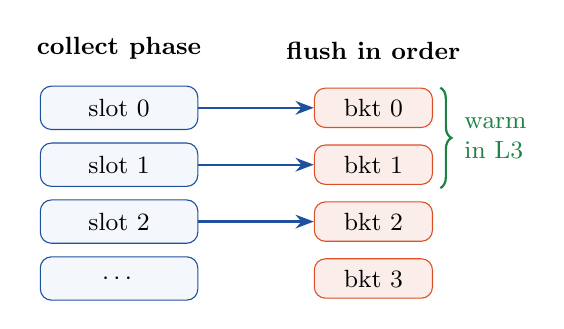
\begin{tikzpicture}[scale=0.85,
  slot/.style={draw=midblue,fill=lightblue!20,rounded corners,
               minimum width=2.0cm,minimum height=0.55cm,font=\small},
  bkt/.style={draw=accent,fill=accent!10,rounded corners,
              minimum width=1.5cm,minimum height=0.5cm,font=\small}]
  % Slots
  \foreach \i/\lbl in {0/slot 0,1/slot 1,2/slot 2,3/$\cdots$}{
    \node[slot] (s\i) at (0,3.2-\i*0.85) {\lbl};}
  \node[above=2pt,font=\small\bfseries] at (0,3.7) {collect phase};
  % EH buckets
  \foreach \i in {0,1,2,3}{
    \node[bkt] (b\i) at (3.8,3.2-\i*0.85) {bkt $\i$};}
  \node[above=2pt,font=\small\bfseries] at (3.8,3.7) {flush in order};
  % arrows
  \foreach \i in {0,1,2}{
    \draw[-Stealth,thick,midblue] (s\i.east) -- (b\i.west);}
  % locality annotation
  \draw[decorate,decoration={brace,amplitude=4pt},thick,dkgreen]
    (4.8,3.5) -- (4.8,2.0) node[midway,right=5pt,font=\small,align=left]{warm\\in L3};
\end{tikzpicture}

\vspace{0.2cm}
\textbf{Cost model:}\\
$N$ output states, $P$ slots:\\
Collect: $N$ writes (sequential per slot)\\
Flush: $N$ reads + 1 DRAM load per bucket\\
$\ll$ 1 DRAM load per \emph{insert}
\end{columns}
\end{frame}

\begin{frame}{Hardware-Adaptive Compile-Time Constants}
\small
\begin{columns}[c]
\column{0.52\textwidth}
Three constants from L1/L2/L3 sizes via \texttt{sysctl} / \texttt{/sys/\ldots/cache/}.

\vspace{0.1cm}
\textbf{Bucket capacity $B$:}
\[
  B = \begin{cases}64 & L_1 \ge 64\,\text{KB}\\32 & \text{otherwise}\end{cases}
\]

\textbf{Rsort threshold $\tau$:} activate when pool $> L_3$
\[
  \tau = 2^{\lfloor\log_2(L_3/\beta)\rfloor}, \quad
  \beta = \tfrac{B \cdot 24 + 8}{B \cdot 0.75}
\]

\textbf{Partition count $P = 2^R$:} flush region $\approx L_2/16$
\[
  R = \operatorname{clamp}\!\!\left(
    \left\lceil\log_2\tfrac{N_{\mathrm{des}}\beta}{L_2/16}\right\rceil,\;
    8, 12\right)
\]

\column{0.44\textwidth}
\begin{center}
\footnotesize
\begin{tabular}{lrrrr}
\toprule
CPU & $L_2$ & $L_3$ & $\tau$ & $R$ \\
\midrule
M3 Pro & 16\,MB & 24\,MB & 512K & 10 \\
M3 base & 16\,MB & 8\,MB & 256K & 10 \\
x86 laptop & 512\,KB & 8\,MB & 128K & 12 \\
Xeon & 256\,KB & 30\,MB & 512K & 12 \\
\bottomrule
\end{tabular}
\end{center}

\vspace{0.15cm}
\begin{exampleblock}{Auto-tuning}
  \texttt{\#ifndef} guards; Python driver detects cache sizes, passes \texttt{-D} flags to \texttt{gcc}.
  New machine $\Rightarrow$ recompiles automatically.
  Portable to Linux (\texttt{MAP\_ANON}/\texttt{MADV\_FREE} supported).
\end{exampleblock}
\end{columns}
\end{frame}

% ==================== PART V: OS MEMORY ====================
{
\setbeamercolor{background canvas}{bg=darkblue}
\begin{frame}[plain]
  \vspace{2cm}
  \begin{center}
    {\color{lightblue}\small Part V}\\[0.4cm]
    {\color{white}\LARGE\bfseries Iteration 4: OS Memory Management}
  \end{center}
\end{frame}
}

\begin{frame}{The malloc/free Trap on macOS}
\small
\begin{columns}[c]
\column{0.52\textwidth}
\textbf{Symptom:} 73--88\,GB swap after 30+ steps of $n=61$, with all prior fixes in place.

\vspace{0.15cm}
\textbf{Root cause:} two pools grow per step:

\vspace{0.05cm}
\textbf{1. Rsort slots:} 50M states $\Rightarrow$ 1.2\,GB/buffer.\\
2 buffers/step $\times$ 33 steps $= \mathbf{79\,GB}$ accumulated.

\vspace{0.05cm}
\textbf{2. EH slabs:} 270M states $\Rightarrow$ 8.7\,GB/EHT.\\
2 EHTs, never freed $= 10$--$20$\,GB.

\vspace{0.15cm}
\begin{alertblock}{The trap}
  \texttt{free()} returns to \emph{allocator heap}, not OS.\\
  Virtual space grows monotonically.\\
  macOS swaps ``freed'' pages rather than unmapping.
\end{alertblock}

\column{0.44\textwidth}
\textbf{Failed: \texttt{madvise(MADV\_FREE)}.}

\vspace{0.1cm}
Advisory on macOS — OS ignores it, especially under the memory pressure when it would matter.

\vspace{0.15cm}
\begin{block}{The correct fix}
  \textbf{Slabs:} \texttt{free(sl->bkts)} in \texttt{eh\_reset()}, \texttt{sl->bkts=NULL}, re-malloc in \texttt{eh\_bkt\_alloc()}.\\[3pt]
  \textbf{Why:} slabs are $\approx 3.2$\,MB — above macOS's threshold for \texttt{mmap}-backed malloc. So \texttt{free()} $\Rightarrow$ \texttt{munmap()} $\Rightarrow$ pages returned unconditionally.\\[3pt]
  \textbf{Rsort:} one flat 480\,MB malloc, reused every step.
\end{block}
\end{columns}
\end{frame}

\begin{frame}{Memory Under Control: Before and After}
\small
\begin{columns}[c]
\column{0.50\textwidth}
\textbf{$n=61$ run (M3 Pro):}

\vspace{0.1cm}
\begin{center}
\begin{tabular}{lrr}
\toprule
Component & Before & After \\
\midrule
EH slabs (curr) & accumulates & freed/step \\
EH slabs (nxt) & accumulates & freed/step \\
Rsort buffer & $\sim$1.2\,GB/step & 480\,MB flat \\
\midrule
Peak RAM & $>$80\,GB swap & \textbf{$<$2\,GB} \\
\bottomrule
\end{tabular}
\end{center}

\vspace{0.15cm}
\textbf{General fix:} allocations $>128$\,KB $\Rightarrow$ malloc uses mmap; \texttt{free()} $\Rightarrow$ \texttt{munmap}.\\
Same misunderstanding affects any long-running loop on macOS.

\column{0.46\textwidth}
\begin{exampleblock}{The FFTW parallel}
  Like FFTW: correct behaviour depends on OS details invisible from C.\\[3pt]
  FFTW probes hardware to pick the best FFT algorithm; we probe the allocator to pick the right memory strategy.
\end{exampleblock}

\vspace{0.1cm}
\begin{block}{Portability}
  Linux: large malloc uses mmap; same \texttt{free()} fix applies.\\
  \texttt{madvise(MADV\_DONTNEED)} also reliable on Linux.
\end{block}
\end{columns}
\end{frame}

% ==================== PART VI: PARALLEL SORT-MERGE ====================
{
\setbeamercolor{background canvas}{bg=darkblue}
\begin{frame}[plain]
  \vspace{2cm}
  \begin{center}
    {\color{lightblue}\small Part VI}\\[0.4cm]
    {\color{white}\LARGE\bfseries Iteration 5: Going Parallel}\\[0.3cm]
    {\color{lightblue}\large Generate, Sort, Merge}
  \end{center}
\end{frame}
}

\begin{frame}{Why the Obvious Parallelisations Failed}
\footnotesize
\begin{columns}[t]
\column{0.50\textwidth}
\textbf{Attempt 1: thread-local hash tables + merge}
\begin{itemize}
  \item Split the scan of \texttt{curr} across threads
  \item Each thread inserts into its own LP table
  \item Main thread re-inserts all local tables into \texttt{nxt}
\end{itemize}
\textbf{Result ($n=45$, 2 threads):} \alert{$1.65\times$ slower} than serial.\\
The serial merge does the same $O(\text{cnt})$ random inserts as the original sweep.

\vspace{0.2cm}
\textbf{Attempt 2: per-worker EH tables}
\begin{itemize}
  \item Merge becomes parallel, but every worker still does
        \alert{random writes} into an 80\,MB table
  \item Two random-access passes per output state
\end{itemize}

\column{0.46\textwidth}
\begin{alertblock}{The lesson}
  Parallelising the \emph{scan} is easy.\\[2pt]
  The hard part is the \emph{reduction}: summing counts of equal keys.\\[2pt]
  A hash table makes the reduction a stream of random writes, and
  sharing it across threads makes it worse.
\end{alertblock}

\vspace{0.2cm}
\begin{block}{The fix}
  Do the reduction by \textbf{sorting}: sequential writes, sequential
  reads, bandwidth-limited rather than latency-limited, and
  splittable into independent pieces.
\end{block}
\end{columns}
\end{frame}

\begin{frame}{Generate $\to$ Sort $\to$ Merge}
\small
\textbf{Key observation:} a source state $(k,c)$ and a subset $S$ of the
$\nb$ back-edges give \emph{at most one} contribution $(k',c)$.
All $|\curr|\cdot 2^{\nb}$ contributions are independent; only the
summation over equal $k'$ couples them.

\vspace{0.15cm}
\begin{center}
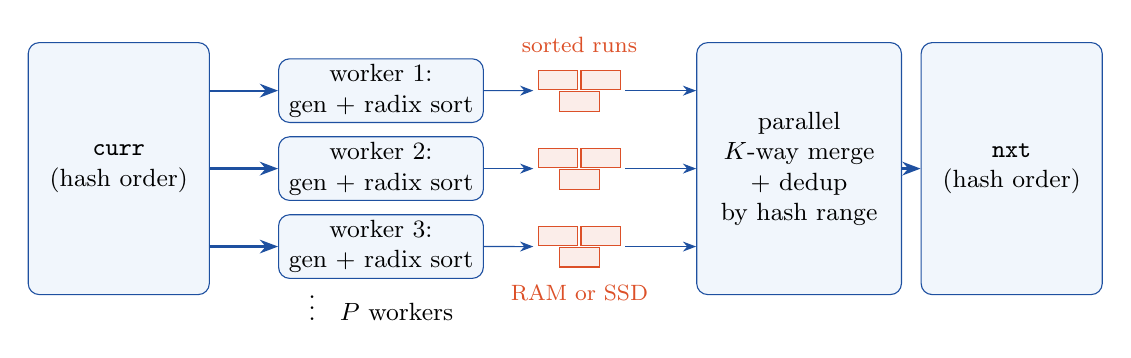
\begin{tikzpicture}[scale=0.9,
  box/.style={draw=midblue,fill=lightblue!25,rounded corners,
              minimum width=2.3cm,minimum height=0.8cm,font=\small,align=center},
  run/.style={draw=accent,fill=accent!10,minimum width=0.5cm,minimum height=0.25cm}]
  \node[box,minimum height=3.2cm] (curr) at (0,0) {\texttt{curr}\\(hash order)};
  \foreach \i/\y in {1/1.1,2/0,3/-1.1}{
    \node[box,minimum width=2.6cm,minimum height=0.7cm,inner sep=2pt] (w\i) at (3.7,\y) {worker \i:\\gen + radix sort};
    \draw[-Stealth,thick,midblue] (curr.east |- w\i.west) -- (w\i.west);
  }
  \node[font=\small] at (3.7,-1.85) {$\vdots$ \; $P$ workers};
  \foreach \i/\y in {1/1.1,2/0,3/-1.1}{
    \node[run] (r\i a) at (6.2,\y+0.15) {};
    \node[run] (r\i b) at (6.8,\y+0.15) {};
    \node[run] (r\i c) at (6.5,\y-0.15) {};
    \draw[-Stealth,midblue] (w\i.east) -- (5.85,\y);
  }
  \node[font=\footnotesize,accent] at (6.5,1.75) {sorted runs};
  \node[font=\footnotesize,accent] at (6.5,-1.75) {RAM or SSD};
  \node[box,minimum height=3.2cm,minimum width=2.6cm] (m) at (9.6,0)
       {parallel\\$K$-way merge\\+ dedup\\by hash range};
  \foreach \y in {1.1,0,-1.1}{\draw[-Stealth,midblue] (7.15,\y) -- (m.west |- 0,\y);}
  \node[box,minimum height=3.2cm] (nxt) at (12.6,0) {\texttt{nxt}\\(hash order)};
  \draw[-Stealth,thick,midblue] (m) -- (nxt);
\end{tikzpicture}
\end{center}

\vspace{0.1cm}
\begin{itemize}
  \item \textbf{No shared writes} in either parallel phase: no atomics on counts, no locks
        (one mutex for the final scalar total)
  \item Introduce of the new vertex is done \textbf{in place} (OR new high bits): saves a full table copy
\end{itemize}
\end{frame}

\begin{frame}{Workers, Runs, and the RAM/SSD Decision}
\small
\begin{columns}[t]
\column{0.52\textwidth}
\textbf{Worker $i$} scans the contiguous slice
$[i\cdot\textit{chunk},\,(i{+}1)\cdot\textit{chunk})$ of \texttt{curr}:
\begin{enumerate}
  \item for each state and each subset $S$: apply edges, apply eliminations,
        append $(k',c)$ to a private buffer
  \item buffer full ($\texttt{CAP}$ entries) $\Rightarrow$ \textbf{flush}:
        8-pass LSD radix sort by $h(k')$, dedup adjacent keys, store as a sorted \emph{run}
\end{enumerate}

\vspace{0.1cm}
\begin{block}{Memory bound}
  Peak during generation:
  \[ |\curr| + P\cdot 2\cdot\texttt{CAP}\cdot 16\,\text{B} \]
  \emph{independent of the output size}.
\end{block}

\column{0.44\textwidth}
\textbf{Per step:} estimate the merge peak
\[
  2\cdot\Bigl\lceil\tfrac{\textit{chunk}\cdot 2^{\nb}}{\texttt{CAP}}\Bigr\rceil
  \cdot \texttt{CAP}\cdot P\cdot 16\,\text{B}
\]
and compare with free RAM.

\vspace{0.1cm}
\begin{itemize}
  \item \textbf{fits:} runs stay in RAM; each worker merges its own runs,
        bucketed by the top byte of $h$ (256 sub-merges that each fit in L2);
        then a parallel $P$-way merge
  \item \textbf{does not fit:} runs are spilled to SSD; one parallel merge of
        \emph{all} runs (up to \textbf{694 streams} at $n=75$), stream buffers sized
        to $\text{SLC}/K$
\end{itemize}
\end{columns}
\end{frame}

\begin{frame}{Parallel Merge by Hash Range}
\small
\begin{columns}[c]
\column{0.52\textwidth}
Given $K$ sorted streams and $T$ threads:
\begin{enumerate}
  \item sample 64 hash values per stream; sort; pick $T{-}1$ splitters
  \item binary-search every stream for every splitter
  \item bound each range's output; give range $r$ its own slice of \texttt{nxt}
  \item thread $r$ heap-merges its $K$ sub-streams with dedup
  \item prefix-sum actual lengths; \texttt{memmove} to close gaps
\end{enumerate}

\vspace{0.15cm}
\begin{exampleblock}{Why dedup stays exact}
  Equal keys $\Rightarrow$ equal hashes $\Rightarrow$ same range.\\
  No two threads ever produce the same key.
\end{exampleblock}

\column{0.44\textwidth}
\centering
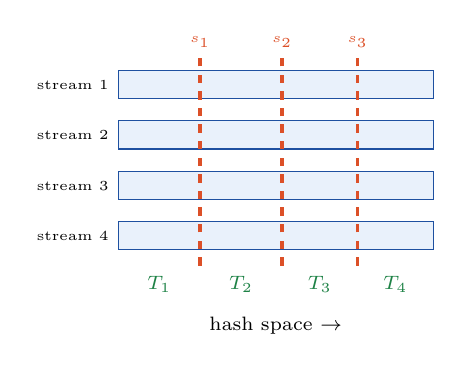
\begin{tikzpicture}[scale=0.8]
  \foreach \s/\y in {1/2.4,2/1.6,3/0.8,4/0}{
    \draw[fill=lightblue!40,draw=midblue] (0,\y) rectangle (5,\y+0.45);
    \node[left,font=\tiny] at (0,\y+0.22) {stream \s};
  }
  \foreach \x/\c in {1.3/accent,2.6/accent,3.8/accent}{
    \draw[\c,very thick,dashed] (\x,-0.25) -- (\x,3.1);
  }
  \node[font=\tiny,accent] at (1.3,3.3) {$s_1$};
  \node[font=\tiny,accent] at (2.6,3.3) {$s_2$};
  \node[font=\tiny,accent] at (3.8,3.3) {$s_3$};
  \foreach \x/\t in {0.65/1,1.95/2,3.2/3,4.4/4}{
    \node[font=\scriptsize,dkgreen] at (\x,-0.55) {$T_{\t}$};
  }
  \node[font=\scriptsize,align=center] at (2.5,-1.2) {hash space $\to$};
\end{tikzpicture}

\vspace{0.1cm}
{\small Splitters are in \emph{hash} space, and the streams are
sorted by hash, so the cuts are consistent across streams.}
\end{columns}
\end{frame}

\begin{frame}{Load Balancing Without a Cost Model}
\footnotesize
\begin{columns}[t]
\column{0.50\textwidth}
\textbf{The difficulty:} the work for a state is the number of subsets $S$
that survive the degree, cycle and elimination checks. It varies by orders
of magnitude, and nothing cheap in the key predicts it.

\vspace{0.15cm}
\begin{block}{The trick: randomise, don't predict}
  Every table is stored in order of $h(k)$, a bijective mixing of the key.
  So a contiguous slice of \texttt{curr} is effectively a \textbf{random sample}
  of states, and static slices balance in expectation.
\end{block}

\vspace{0.1cm}
\textbf{$n=75$, 64 workers:} slowest / mean worker time

\vspace{0.05cm}
{\scriptsize
\setlength{\tabcolsep}{4pt}
\begin{tabular}{l*{6}{r}}
\toprule
step & 30 & 36 & 42 & 46 & 56 & 60\\
\midrule
max/mean & 1.03 & 1.19 & 1.17 & 1.18 & 1.17 & 1.13\\
\bottomrule
\end{tabular}}

Light steps reach 1.5--1.9, but they are short.

\column{0.46\textwidth}
\begin{alertblock}{The bug that proved the point}
  An earlier version radix-sorted by the \emph{raw} key but chose merge
  splitters in \emph{hash} space.\\[3pt]
  Raw keys have top byte \texttt{0x80} or \texttt{0xC0} only (flag bits):
  all entries in 2 of 256 buckets.\\[3pt]
  Splitters meaningless $\Rightarrow$ \textbf{5 of 6 merge threads idle}
  (10\% CPU at $n=61$), and wrong bucket boundaries in the RAM merge.
\end{alertblock}

\vspace{0.1cm}
\textbf{Also:}
\begin{itemize}
  \item per-worker state padded to a 128-byte line: false sharing on
        \texttt{buf\_len} cost $3$--$4\times$
  \item a work-stealing queue was written \emph{and never needed}
\end{itemize}
\end{columns}
\end{frame}

\begin{frame}{Correctness Hazards at Scale}
\footnotesize
\begin{columns}[t]
\column{0.50\textwidth}
\textbf{Silent data loss under memory pressure}
\begin{itemize}
  \item Spilled runs lived in \texttt{MAP\_ANON} pages marked \texttt{MADV\_FREE}
  \item Under pressure the OS reclaimed them; later reads returned \alert{zeros}
  \item Zero keys sort below every valid bucket and were \alert{skipped}:
        wrong count, no error
  \item Fix: never \texttt{MADV\_FREE} live data; size the backing store for the
        worst case; file-backed storage when RAM is short
\end{itemize}

\vspace{0.1cm}
\textbf{The 64-bit boundary}
\begin{itemize}
  \item Entries shrunk 24\,B $\to$ 16\,B by making counts \texttt{u64}
        (totals stay \texttt{u128})
  \item every addition checks wraparound; a global flag
        $\Rightarrow$ \texttt{OverflowError}
\end{itemize}

\column{0.46\textwidth}
\begin{block}{Cross-checks that passed}
  \begin{itemize}
    \item SM vs EH agree on all small $n$ (smoke tests to $n=47$)
    \item Linux SM runs for $n=57$--$61$ reproduce the laptop EH values
    \item $n=74$: \textbf{four} runs (same ordering, two code versions,
          DP time 945--3449\,s) give the same count
  \end{itemize}
\end{block}

\vspace{0.1cm}
\begin{alertblock}{$n=75$: the April value was wrong}
  First frontier of width 15: 16 slots during a step, but the old key had
  15 slots + 2 flag bits, so slot 16 overlapped the flags. Fixed key: 16 slots,
  no flags. Two orderings now agree on $9.23\cdot10^{18}$.
\end{alertblock}
\end{columns}
\end{frame}

\begin{frame}{Effect of Pruning on Time and Storage}
\footnotesize
\begin{columns}[t]
\column{0.40\textwidth}
Pruning dead states (Du's idea; see the algorithm talk) is applied by the
workers after the eliminations, \emph{before} a contribution enters a
buffer: a dead state is never sorted, merged, stored or extended.
Cost per key: a few popcounts and a bit-set fix-point.

\vspace{0.15cm}
\textbf{Why sort and merge gain most:} without pruning, 11 steps no longer
fit in 18\,GB and spill runs to SSD (up to 25\,GB).

\vspace{0.1cm}
\textbf{Why peak RSS gains least:} the worker buffers
($2P\cdot\texttt{CAP}$ = 6.4\,GB) are the same in both runs.

\vspace{0.1cm}
\textbf{Gain grows with $n$:} $1.5$--$2.3\times$ at $n=55$--$57$ (4-thread VM).

\column{0.56\textwidth}
\textbf{$n=61$}, M3 Pro 18\,GB, 6 threads, same build and ordering

\vspace{0.05cm}
\begin{center}
\begin{tabular}{lrrr}
\toprule
 & without & with & \\
\midrule
\rowcolor{dkgreen!15}
DP time & 1177\,s & 282\,s & $4.2\times$\\
\quad generate & 773\,s & 228\,s & $3.4\times$\\
\quad sort (flush) & 236\,s & 32\,s & $7.4\times$\\
\quad merge & 182\,s & 21\,s & $8.7\times$\\
\midrule
states, all steps & 6.52\,G & 1.50\,G & $4.4\times$\\
largest table & 702\,M & 144\,M & $4.9\times$\\
\quad as 16\,B entries & 11.2\,GB & 2.3\,GB & \\
steps spilling to SSD & 11 & 0 & \\
peak RSS & 12.1\,GB & 8.7\,GB & $1.4\times$\\
\bottomrule
\end{tabular}
\end{center}
Single runs; counts identical (3711439128718).
\end{columns}
\end{frame}

% ==================== PART VII: RESULTS ====================
{
\setbeamercolor{background canvas}{bg=darkblue}
\begin{frame}[plain]
  \vspace{2cm}
  \begin{center}
    {\color{lightblue}\small Part VII}\\[0.4cm]
    {\color{white}\LARGE\bfseries Results and Lessons}
  \end{center}
\end{frame}
}

\begin{frame}{Full Performance Progression for $n=58$}
\small
\begin{columns}[c]
\column{0.52\textwidth}
\textbf{Same problem, M3 Pro unless noted:}

\vspace{0.1cm}
\begin{center}
\begin{tabular}{lrr}
\toprule
Version & Time & Memory \\
\midrule
LP (no buffer) & 265.8\,s & $\sim$3\,GB \\
LP + write buffer & 149.4\,s & $\sim$3\,GB \\
EH (no rsort) & 163.8\,s & $\sim$3\,GB \\
EH + rsort buffer & 148.7\,s\,{\small(M3)} & accumulates \\
\rowcolor{dkgreen!15}
EH + rsort + free & 117.4\,s & \textbf{$<$2\,GB} \\
\bottomrule
\end{tabular}
\end{center}

\vspace{0.1cm}
$1.78\times$ over unoptimised LP. Memory fix also improves speed: freed pages reduce cache pressure.

\vspace{0.1cm}
\textbf{BW validation:} M3/M3 Pro ratio $1.497\times$ (spec $1.50\times$, 0.3\% error).

\column{0.44\textwidth}
\textbf{At $n=59$ and $n=61$:}

\vspace{0.1cm}
\begin{center}
\begin{tabular}{lrr}
\toprule
$n$ & LP & EH+free \\
\midrule
58 & 149.4\,s & 117.4\,s \\
59 & 1401\,s & 510\,s \\
\rowcolor{accent!10}
59 step 38 & 853\,s & 160\,s \\
\midrule
61 & (OOM) & \textbf{97\,min} \\
\bottomrule
\end{tabular}
\end{center}

\vspace{0.1cm}
$n=59$: \textbf{2.75$\times$} end-to-end; step 38: \textbf{5.3$\times$}.\\
$n=61$: LP OOM; EH+free finishes in 97\,min.\\
{\small Peak $n=61$: 620M states; $<$2\,GB RAM throughout.}
\end{columns}
\end{frame}

\begin{frame}{$n=61$: Step Profile}
\small
\begin{columns}[c]
\column{0.50\textwidth}
\textbf{Double-peak structure:}

\vspace{0.1cm}
\begin{center}
\footnotesize
\begin{tabular}{rrrrrr}
\toprule
Step & $f_s$ & $\nb$ & In & Out & Time \\
\midrule
34 & 14 & 4 & 236M & 441M & 503\,s \\
\rowcolor{accent!15}
35 & 14 & 2 & 441M & 502M & 450\,s \\
\rowcolor{accent!20}
36 & 14 & 3 & 502M & \textbf{620M} & \textbf{1481\,s} \\
37 & 13 & 2 & 620M & 142M & 960\,s \\
38 & 13 & 1 & 142M & 115M & 48\,s \\
\rowcolor{accent!15}
39 & 14 & 3 & 115M & 466M & 740\,s \\
40 & 13 & 3 & 466M & 143M & 636\,s \\
\midrule
\multicolumn{5}{l}{Total} & 97\,min \\
\bottomrule
\end{tabular}
\end{center}

\column{0.46\textwidth}
\begin{itemize}
  \item Step 36: \textbf{25\% of total runtime}
  \item Steps 36+37+39+40: \textbf{65\% of total}
  \item Two peaks at steps 36 and 39 — pw=14 threading a topologically complex region of $G_{61}$
  \item Step 51 (51M$\to$156K): frontier collapses as eliminations cascade
\end{itemize}

\vspace{0.15cm}
\begin{block}{New result}
  $|\mathrm{Ham}(G_{61})| = \mathbf{3{,}711{,}439{,}128{,}718}$\\[2pt]
  First time computed.\\
  Previous: $|\mathrm{Ham}(G_{57})| = 68\times10^9$.
\end{block}
\end{columns}
\end{frame}

\begin{frame}{Sort--Merge Results: $n\le 75$ on 768\,GB / 64 Cores}
\footnotesize
\begin{columns}[c]
\column{0.56\textwidth}
\centering
{\scriptsize
\renewcommand{\arraystretch}{0.92}
\begin{tabular}{rrrr}
\toprule
$n$ & width & $|\mathrm{Ham}(G_n)|$ & DP time \\
\midrule
61 & 14 & 3{,}711{,}439{,}128{,}718 & 699\,s \\
62 & 14 & 19{,}133{,}360{,}717{,}991 & 1049\,s \\
63 & 14 & 121{,}460{,}168{,}051{,}419 & 1162\,s \\
64 & 14 & 329{,}054{,}896{,}751{,}390 & 1551\,s \\
65 & 14 & 780{,}444{,}607{,}816{,}976 & 1643\,s \\
66 & 14 & 1{,}389{,}466{,}102{,}344{,}323 & 1858\,s \\
67 & 14 & 2{,}317{,}807{,}210{,}864{,}530 & 1742\,s \\
68 & 14 & 5{,}019{,}822{,}900{,}252{,}036 & 2167\,s \\
69 & 14 & 6{,}697{,}388{,}275{,}608{,}246 & 1465\,s \\
70 & 14 & 12{,}684{,}480{,}251{,}402{,}254 & 1635\,s \\
71 & 14 & 65{,}830{,}124{,}660{,}217{,}873 & 2795\,s \\
72 & 14 & 132{,}407{,}660{,}925{,}860{,}729 & 2418\,s \\
73 & 14 & 536{,}884{,}024{,}745{,}221{,}467 & 2079\,s \\
74 & 14 & 2{,}176{,}025{,}661{,}130{,}535{,}741 & 3449\,s \\
\rowcolor{accent!12}
75 & 15 & 9{,}231{,}885{,}593{,}047{,}053{,}408$^\dagger$ & 1047\,s \\
\bottomrule
\end{tabular}}

\vspace{0.05cm}
{\tiny $^\dagger$ current code with pruning; a second ordering ($V_7$, 963\,s) gives the same count; the April value was withdrawn. DP time excludes the ordering
(MaxSAT + annealing: 5--37\,min). $n\le 74$: April 13 code. Later code (in-place
introduce, 16-byte entries) did $n=74$ in 945\,s.}

\column{0.40\textwidth}
\textbf{Scale}
\begin{itemize}
  \item width 14: peak $\approx 8\cdot10^8$ states, 0--3 steps spilled to SSD
  \item width 15 ($n=75$, with pruning): peak $1.2\cdot10^9$ states,
        nothing spilled
\end{itemize}

\vspace{0.1cm}
\textbf{Same algorithm, two machines}
\begin{itemize}
  \item $n=59$, M3 Pro: SM 317\,s vs best EH 385\,s
  \item $n=61$: laptop EH 97\,min; server SM 12\,min
\end{itemize}

\vspace{0.1cm}
\begin{exampleblock}{$n=75$ confirmed}
  Two optimal orderings (differing in 71 of 75 positions) give the same count.
  $H(75)/H(74)\approx 4.24$ (the withdrawn April value gave $\approx 300$).
\end{exampleblock}
\end{columns}
\end{frame}

\begin{frame}{Storage Hierarchy Lessons}
\small
\begin{columns}[t]
\column{0.48\textwidth}
\textbf{\color{midblue}Lesson 1: Proportional allocation wins}

EH sizes its table to \emph{actual output}, not estimated input.
Eliminated pre-allocation waste and three-table spike.
The 1979 disk-page design maps directly to DRAM-to-L3.

\vspace{0.15cm}
\textbf{\color{midblue}Lesson 2: Locality must be enforced, not hoped for}

Random writes will miss the cache. No pre-fetching fixes this —
you must \emph{reorder} the writes. The radix-sort buffer gives a
1-DRAM-load-per-bucket guarantee by construction.

\vspace{0.15cm}
\textbf{\color{midblue}Lesson 3: madvise is not free()}

\texttt{MADV\_FREE} on \texttt{malloc}-backed memory is advisory on macOS.
Use \texttt{free()} on allocations $>128$\,KB to trigger \texttt{munmap}.

\column{0.48\textwidth}
\textbf{\color{midblue}Lesson 4: Profile at the right granularity}

Per-step profiling found 65\% of $n=61$ runtime in 4 steps.
Optimising the common case would have been misleading.

\vspace{0.15cm}
\textbf{\color{midblue}Lesson 5: Hardware spec $\approx$ measured ratio}

M3\,/\,M3 Pro per-step ratio: $1.497\times$ (spec: $1.50\times$).
For memory-bound code, bandwidth is the right predictor —
benchmark on a smaller machine and project accurately.

\vspace{0.15cm}
\textbf{\color{midblue}Lesson 6: Engineering compounds}

The gains interact: EH's proportional allocation only matters
because rsort makes inserts fast; the OS fix only matters
because EH accumulates enough slabs to overflow RAM.
\end{columns}
\end{frame}

\begin{frame}{Lessons from Going Parallel}
\footnotesize
\begin{columns}[t]
\column{0.48\textwidth}
\textbf{\color{midblue}Lesson 7: Reduce by sorting, not hashing}

Once there are many threads, a shared or per-thread hash table makes the
reduction a stream of random writes. Sorted runs turn it into sequential
bandwidth, bounded buffers, and a merge that splits cleanly.

\vspace{0.15cm}
\textbf{\color{midblue}Lesson 8: Balance by randomising}

Per-state work could not be predicted from the key. Storing every table in
hash order made static slices balanced to within 20\% on the steps that matter.
The work-stealing queue was never needed.

\vspace{0.15cm}
\textbf{\color{midblue}Lesson 9: Sort and split in the same order}

The raw-key bug idled five of six threads and broke bucket boundaries;
correct answers were luck. Every comparison, bucket and splitter must use
the same order.

\column{0.48\textwidth}
\textbf{\color{midblue}Lesson 10: The OS is part of the algorithm}

\texttt{MADV\_FREE} on live data gave zeros and a wrong count, not a crash.
On the big machine, the run finished only after hand-tuning
\texttt{machine.yaml} (thread count, buffer caps, stream buffers) to the
memory actually available.

\vspace{0.15cm}
\textbf{\color{midblue}Lesson 11: An answer at a new boundary is a conjecture}

$n=75$ was the first width-15 frontier, and its first answer was wrong:
16 slots were needed during a step, and slot 16 overlapped the key's flag bits.
Width-16 tests against Held--Karp now guard this path, and two optimal
orderings agree on the corrected count.
\end{columns}
\end{frame}

% ==================== FINAL ====================
{
\setbeamercolor{background canvas}{bg=darkblue}
\begin{frame}[plain]
  \vspace{0.4cm}
  \begin{center}
    {\color{white}\Large\bfseries Thank You}\\[0.5cm]
    {\color{lightblue}Questions?}\\[0.5cm]

    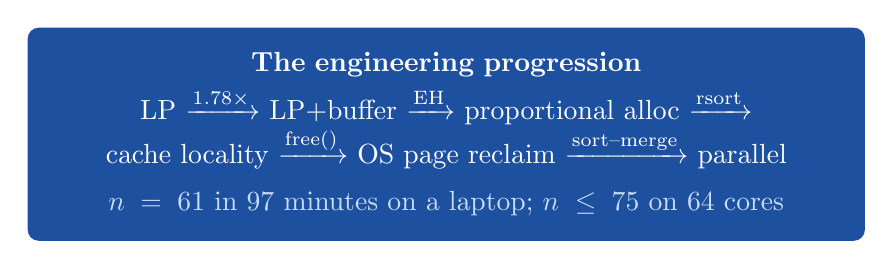
\begin{tikzpicture}
    \node[fill=midblue,rounded corners,inner sep=9pt,text=white,
          text width=10cm,align=center]{
      \textbf{The engineering progression}\\[3pt]
      LP $\xrightarrow{1.78\times}$ LP+buffer $\xrightarrow{\text{EH}}$ proportional alloc
      $\xrightarrow{\text{rsort}}$ cache locality
      $\xrightarrow{\text{free()}}$ OS page reclaim
      $\xrightarrow{\text{sort--merge}}$ parallel\\[5pt]
      \textcolor{lightblue}{$n=61$ in 97 minutes on a laptop; $n\le 75$ on 64 cores}};
    \end{tikzpicture}

    \vspace{0.4cm}
    {\color{lightblue!80}\small
    Code: frontier DP in C via cffi $\cdot$ extendible hashing $\cdot$
    radix-sort buffer $\cdot$ parallel sort--merge $\cdot$ hardware-adaptive constants}\\[0.2cm]
    {\color{lightblue!60}\small
    With thanks to Claude (Anthropic) for algorithm design, profiling, and implementation.}
  \end{center}
\end{frame}
}

\end{document}
